% !Mode:: "TeX:UTF-8"

\chapter{程序结果分析}

%\emph{TODO}: 按通信量与计算时间的比例大小分类、按拓扑结构分类(消息拥塞)、按时间与数据依赖的相对多少分类

%本节通过几个例子分别验证 COSS 算法的流程、处理器排序优化、目标平台的连接对调度结果的影响等,分析几种不同类型任务集的调度结果。
本节通过例子来具体演示 COSS 算法的流程,并分析调度结果在时间约束、数据约束以及子依赖约束等方面的正确性。
\section{算法流程示例}

%\emph{TODO: 给出一个具体例子的输入输出,并结合例子分析说明}

例如有周期任务 A 和 B,运行时间分别为 $C_1=1$ 和 $C_2=2$,周期性时间属性分别为:
\begin{gather*}
  T_A=2, O_A=0, D_A=2 \\
  T_B=3, O_B=0, D_B=3
\end{gather*}
且 A、B 任务之间具有如图 \ref{program-fig-sample-SDF} 所示的通信关系。即任务 A 每次执行向 B 发送 2 个数据,任务 B 每次执行需要消耗由 A 发来的 3 个数据,初始时 B 有 3 个数据可用。由此通信关系造成的数据依赖约束如图中右侧关系所示,任务 B 的第 1 次执行需要受 A 第 1 次运行结束的制约,B 的第 2 次执行受到 A 第 2 次运行结束的制约。

\begin{figure}[!hbt]
  \centering
  % Requires \usepackage{graphicx}
  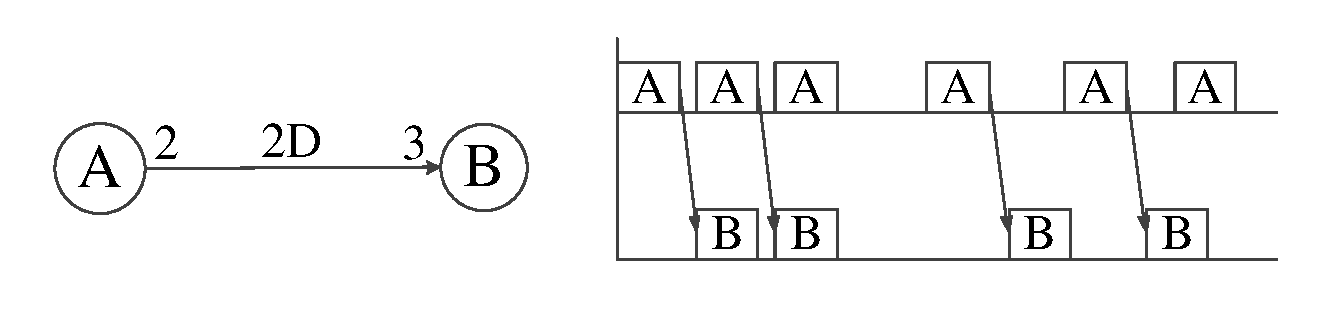
\includegraphics[height=12ex]{figure/program-sample-SDF.pdf}\\
  \caption{A、B 任务之间的通信关系}\label{program-fig-sample-SDF}
\end{figure}

假设将 A、B 调度到由两个处理器组成的目标平台,其连接矩阵为
$$C=\begin{bmatrix}-1 & 1 \\ 1 & -1\end{bmatrix}$$
处理器间通信速率 $s=10$,表示每单位时间从一个处理器向另一个处理器可发送 10 个单位的数据。根据附录所述输入格式,将其整理为如下输入文件:%如表\ref{program-tab-input} 所示。
%{\renewcommand{\arraystretch}{1.5}
%\begin{table}
%  \centering
%  \caption{输入文件示例}
%  \label{program-tab-input}
%  \begin{tabular}{r|l|l}
%    \hline
%      行号 & 文件内容 & 说明\\
%    \hline
%      1 & 2 & 任务数\\
%      2 & 1 2 0 2 -1 & 任务 A 的时间属性\\
%      3 & 2 3 0 3 -1 & 任务 B 的时间属性\\
%      4 & 1 & 任务间数据依赖的个数\\
%      5 & 1 2 2 3 2 & 数据依赖关系\\
%      6 & 1 & 周期倍数\\
%      7 & 2 & 处理器个数\\
%      8 & 10 & 消息传输速率\\
%      9 & 1 & 连接数\\
%      10 & 1 2 & 处理器间连接\\
%    \hline
%  \end{tabular}
%\end{table}
%}
\begin{Verbatim}[numbers=left,frame=single,xleftmargin=50pt,
samepage=true,fontsize=\small,baselinestretch=1.2]
2
1 2 0 2 -1
2 3 0 3 -1
1
1 2 2 3 2
1
2
10
1
1 2
\end{Verbatim}

其中第一行数字 2 表示任务个数,下面 2 行分别表示任务 A 和 B 的时间约束,每行最后的数字 -1 表示该任务不是自依赖的,即没有数据需要在同任务的相邻两次执行之间传递。第四行的数字 1 表示任务间通信关系的个数,下面 1 行表示任务 A、B 之间的具体通信关系。第六行数字 1 表示周期倍数,第七行数字 2 表示目标平台的处理器个数,下面的数字 10 表示处理器之间的通信速率。第九行数字 1 表示处理器之间的连接数,最后 1 行表示哪两个编号的处理器之间有链路相连。

模拟程序按以上信息调度,输出内容分为求解拓扑矩阵、DAG、生成的静态路由表、调度表等几部分。

程序输出拓扑矩阵为:
\begin{equation*}
  \Gamma=\begin{bmatrix}
    1 & -2 & 0 \\
    1 & 0 & -3 \\
    -1 & 2 & 0 \\
    0 & 2 & -3 \\
    -1 & 0 & 3
  \end{bmatrix}
\end{equation*}

由输入任务的时间属性以及任务间的通信关系,用第\ref{chapter-SDF}章介绍的方法,可以构建 GSDF 如图\ref{EXP-fig-GSDF} 所示。考虑到矩阵第1列对应虚拟结点V,第2 列对应任务结点A,第3列对应任务结点B,矩阵的每一行分别对应从 V 到 A 的弧、从 V 到 B 的弧、从 A 到 B 的弧、从 A 到 V 的弧以及从 B 到 V 的弧。可以看到,以上拓扑矩阵与任务 A、B 构建的 GSDF 相符。

\begin{figure}[!hbt]
  \centering
  % Requires \usepackage{graphicx}
  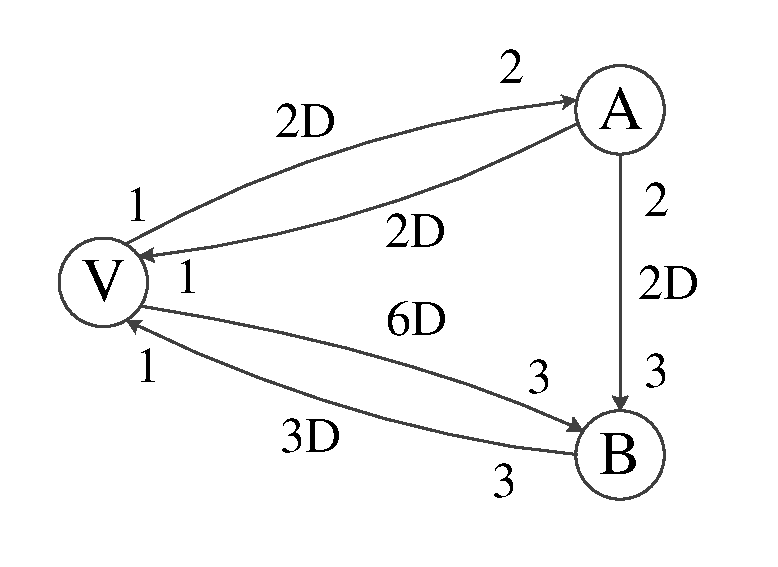
\includegraphics[height=20ex]{figure/EXP-GSDF.pdf}\\
  \caption{A、B 任务构建的 GSDF}\label{EXP-fig-GSDF}
\end{figure}

程序求出以上拓扑矩阵零空间向量的最小整数解为

\begin{equation*}
  q=\begin{bmatrix}
    6 \\
    3 \\
    2
  \end{bmatrix}
\end{equation*}

由以上 GSDF 和 q 构建 DAG,程序输出如下:
\begin{Verbatim}[numbers=left,frame=single,xleftmargin=50pt,
samepage=true,fontsize=\small,baselinestretch=1.2]
======== DAG ========
Task 1:
  (1, 0): (0 2) 0; (2 0) 1; (2 1) 1;
  (1, 1): (0 4) 0; (2 1) 2;
  (1, 2): NP (0 0) 0; NP (0 1) 0; NP (2 0) 2;

Task 2:
  (2, 0): (0 3) 0;
  (2, 1): NP (0 0) 0; NP (0 1) 0; NP (0 2) 0;
\end{Verbatim}

其中 Task 0 表示虚拟任务 V,Task 1 表示任务 A,Task 2 表示任务 B。 任务 i 的第 j 次运行以一对整数 (i, j) 表示,每一行对应从 (i, j) 发出的,向其他任务结点发送的通信信息以及传输数据量。如 (1, 0): (2 0) 1 表示任务 1 的首次运行会向任务 2 的首次运行发送 1 的数据量。如果数据量为 0,表明任务间仅有时间上的制约关系,没有实际的数据通信,这种情况多发生于周期性任务与虚拟任务结点之间。
输出信息中的 NP 表示跨周期结点间的消息传输目标与数据传输量。以上一个调度周期的 DAG 可以表示为图 \ref{EXP-fig-DAG} 所示,其中 $A_2$ 与 $B_0$ 结点间表示跨周期结点间的消息。 图中弧上的数字表示结点间的通信数据量,结点旁的数字为该结点的 SBL 值。从图中可以看出,任务间的通信消息(包括调度周期内和周期间)一共有 4 条。

\begin{figure}[!hbt]
  \centering
  % Requires \usepackage{graphicx}
  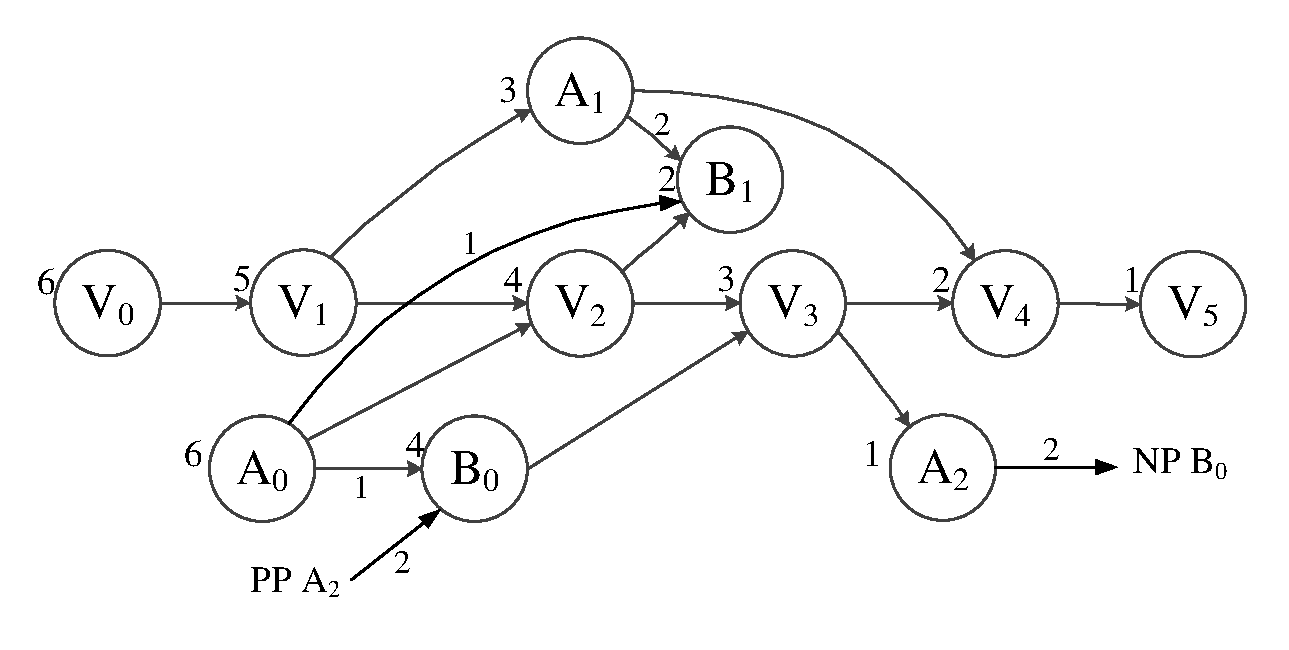
\includegraphics[height=28ex]{figure/EXP-DAG.pdf}\\
  \caption{A、B 任务构建的 DAG}\label{EXP-fig-DAG}
\end{figure}


目标平台是仅有两个核心的处理器,因此路由表非常简单,链路也只有一条,程序输出的下一跳矩阵为
$$H=\begin{bmatrix}-1 & 2\\ 1 & -1\end{bmatrix}$$
最终根据以上 DAG
得到的调度结果为:
\begin{Verbatim}[numbers=left,frame=single,xleftmargin=50pt,
samepage=true,fontsize=\small,baselinestretch=1.2]
===== Schedules =====
Processor 1:
     0.00 -->  1.00: Task (1 0), time 1
     1.00 -->  3.00: Task (2 0), time 2
     4.00 -->  5.00: Task (1 2), time 1

Processor 2:
     2.00 -->  3.00: Task (1 1), time 1
     3.00 -->  5.00: Task (2 1), time 2

Link 1 --- 2:
     1.00 -->  1.10: Task (1 0) --> (2 1), Processor 1 --> 2, data 1

  ---- Task ----
Task 1:
    (1 0): [Processor   1] time  0.00 -->  1.00
    (1 1): [Processor   2] time  2.00 -->  3.00
    (1 2): [Processor   1] time  4.00 -->  5.00

Task 2:
    (2 0): [Processor   1] time  1.00 -->  3.00
    (2 1): [Processor   2] time  3.00 -->  5.00
\end{Verbatim}
由调度结果可以看出,Task 1 的 3 次运行分别在 [0.0, 2.0)、[2.0, 4.0)、[4.0, 6.0) 的时间范围内,Task 2 的 2 次运行分别在 [0.0, 3.0)、[3.0, 6.0)] 的时间范围内,他们的周期性时间约束得到了保证。通信约束方面,Task 2 的第一次执行 (2 0) 是在 [1.0, 3.0) 时段,在 Task 1 的第一次运行 (1 0) 结束后,两者位于同一处理器核心,因此链路上没有这条消息调度。Task 2 的第 2 次执行 (2 1) 是 [3.0, 5.0) 时段,也在 Task 1 的第 2 次执行 ([2, 3] 时段) 结束后,因此周期内的优先关系制约得到了满足,且这两次执行均处于同一处理器,因此也不需在链路上进行消息调度。而 Task 2 的第 2 次执行 (2 1) 需要从 Task 1 第 1 次执行 (1 0) 得到数据,因此在链路上有这条消息的调度。最后,任务 1 的第三次执行 (1 2) 需要向下一周期任务 2 的第一次执行 (2 0) 发送 2 数据的消息,而从调度表可以看出这两者都位于处理器1,因此链路上也无需对这条消息调度。以上调度如图 \ref{EXP-fig-sch1} 所示。

\begin{figure}[!hbt]
  \centering
  % Requires \usepackage{graphicx}
  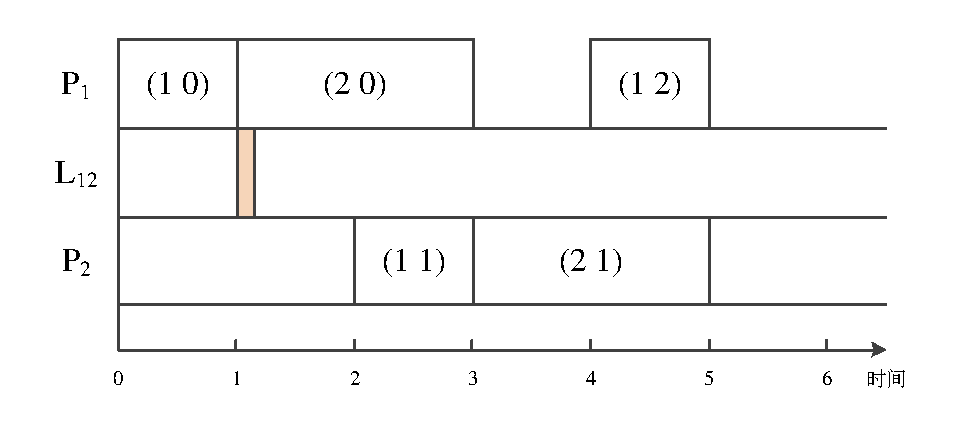
\includegraphics[height=25ex]{figure/EXAMP-sch1.pdf}\\
  \caption{简单例子的调度图}\label{EXP-fig-sch1}
\end{figure}

经过以上分析可以看到,两个任务均在时间限制约束的范围内,且满足了 A、B 之间数据通信的关系。其跨核的消息调度也得以体现。

%\section{处理器排序对调度结果的影响}
%在第 \refl{DLS-processor-sort} 节我们讨论了通过对处理器排序来优化调度结果,使任务更倾向于分配在连接数较多的处理器上,

\section{任务自依赖约束的验证}

为了验证任务自依赖属性对调度结果的影响,下面考虑由六个任务组成的任务集,其任务的时间约束如表\ref{EXP-table-6task-time} 所示,其任务间的数据通信关系如图\ref{EXP-fig-6task-SDF}所示。可以看到六个任务分成了两组各自连通的 SDF 图,其调度关系通过任务的时间约束联系起来。
{\renewcommand{\arraystretch}{1.5}
\begin{table}
  \centering
  \caption{6个任务的时间约束}
  \label{EXP-table-6task-time}
  \begin{tabular}{|c|c|c|c|c|c|}
    \hline
    % after \\: \hline or \cline{col1-col2} \cline{col3-col4} ...
    任务 & 最坏执行时间$C_i$ & 周期$T_i$ & 偏移$O_i$ & 时间限$D_i$ & 自依赖\\
    \hline
    1 & 25 & 60 & 0 & 60 & 否\\
    2 & 30 & 0 & 0 & 0 & 否\\
    3 & 20 & 45 & 0 & 45 & 否\\
    4 & 15 & 0 & 0 & 0 & 否\\
    5 & 10 & 60 & 20 & 30 & 否\\
    6 & 30 & 0 & 0 & 0 & 否\\
    \hline
  \end{tabular}
\end{table}
}
\begin{figure}[!hbt]
  \centering
  % Requires \usepackage{graphicx}
  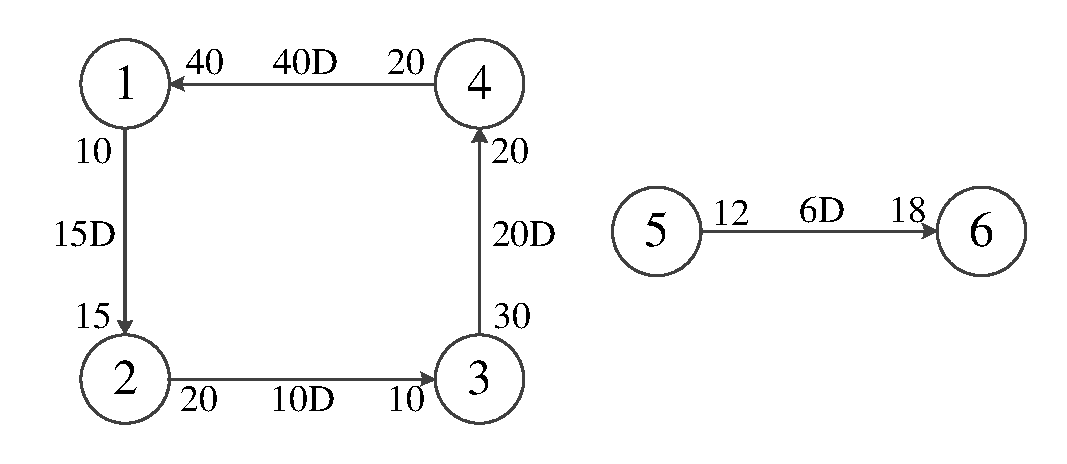
\includegraphics[height=24ex]{figure/EXP-6task-SDF.pdf}\\
  \caption{6个任务的 SDF 图}\label{EXP-fig-6task-SDF}
\end{figure}

调度的目标平台由三个处理器组成,其中处理器1和2相连,2和3相连。另外,为了明确反应数据通信延迟对调度所造成的影响,处理器之间的数据传输速率设为每单位时间1 个数据。我们调用算法模拟程序,可以得到如图\ref{EXP-fig-6task-sched1} 所示的调度结果。由于在表\ref{EXP-table-6task-time} 中所有任务都不是自依赖的,即同一任务在周期内的多次执行不必是串行的,可以看到以下调度图中任务4的几次运行中 (4,0) 和 (4,1) 在时间上有相互重叠的部分,(4,4) 和 (4,5) 也有重叠的部分。如果我们改变任务参数,将任务 4 改为自依赖的,其相邻两次执行之间需要传递10单位的数据,则调度图成为图\ref{EXP-fig-6task-sched2} 所示的结果。
\begin{figure}[!hbt]
  \centering
  % Requires \usepackage{graphicx}
  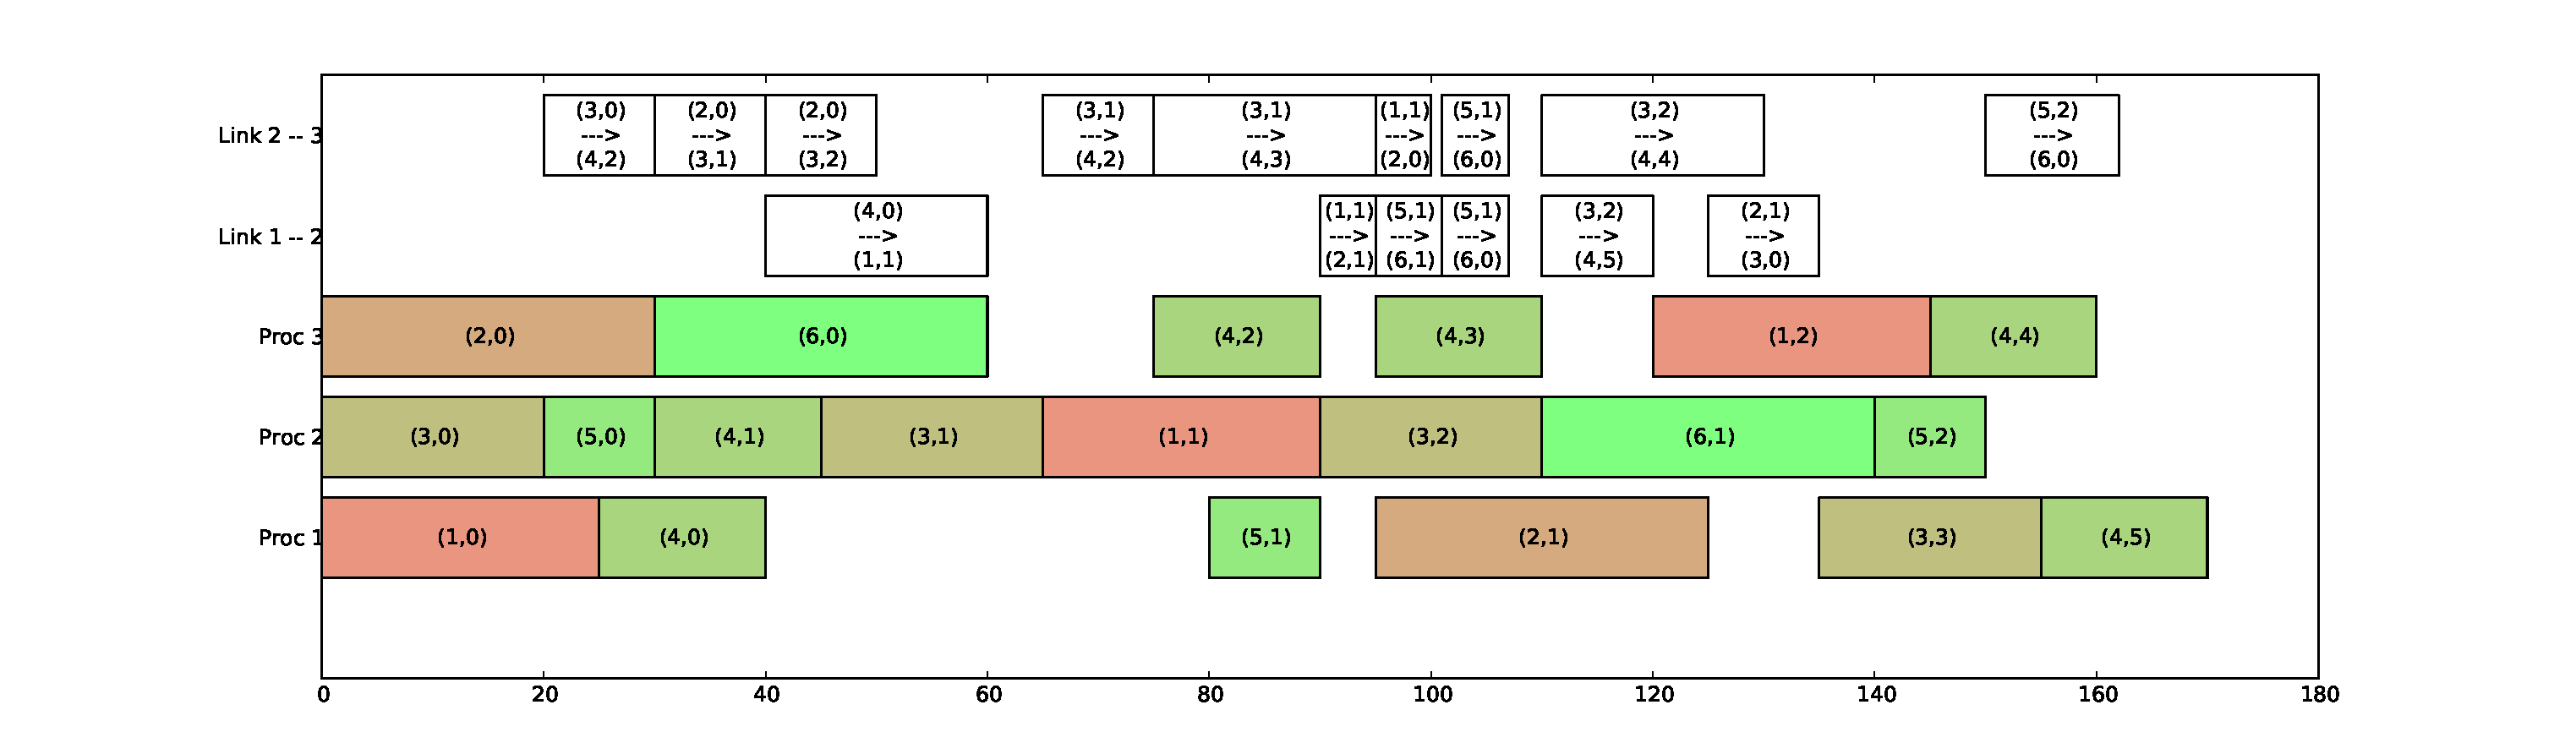
\includegraphics[width=40em]{figure/EXP-6task-sched1.pdf}\\
  \caption{6 个任务的调度表}\label{EXP-fig-6task-sched1}
\end{figure}
\begin{figure}[!htb]
  \centering
  % Requires \usepackage{graphicx}
  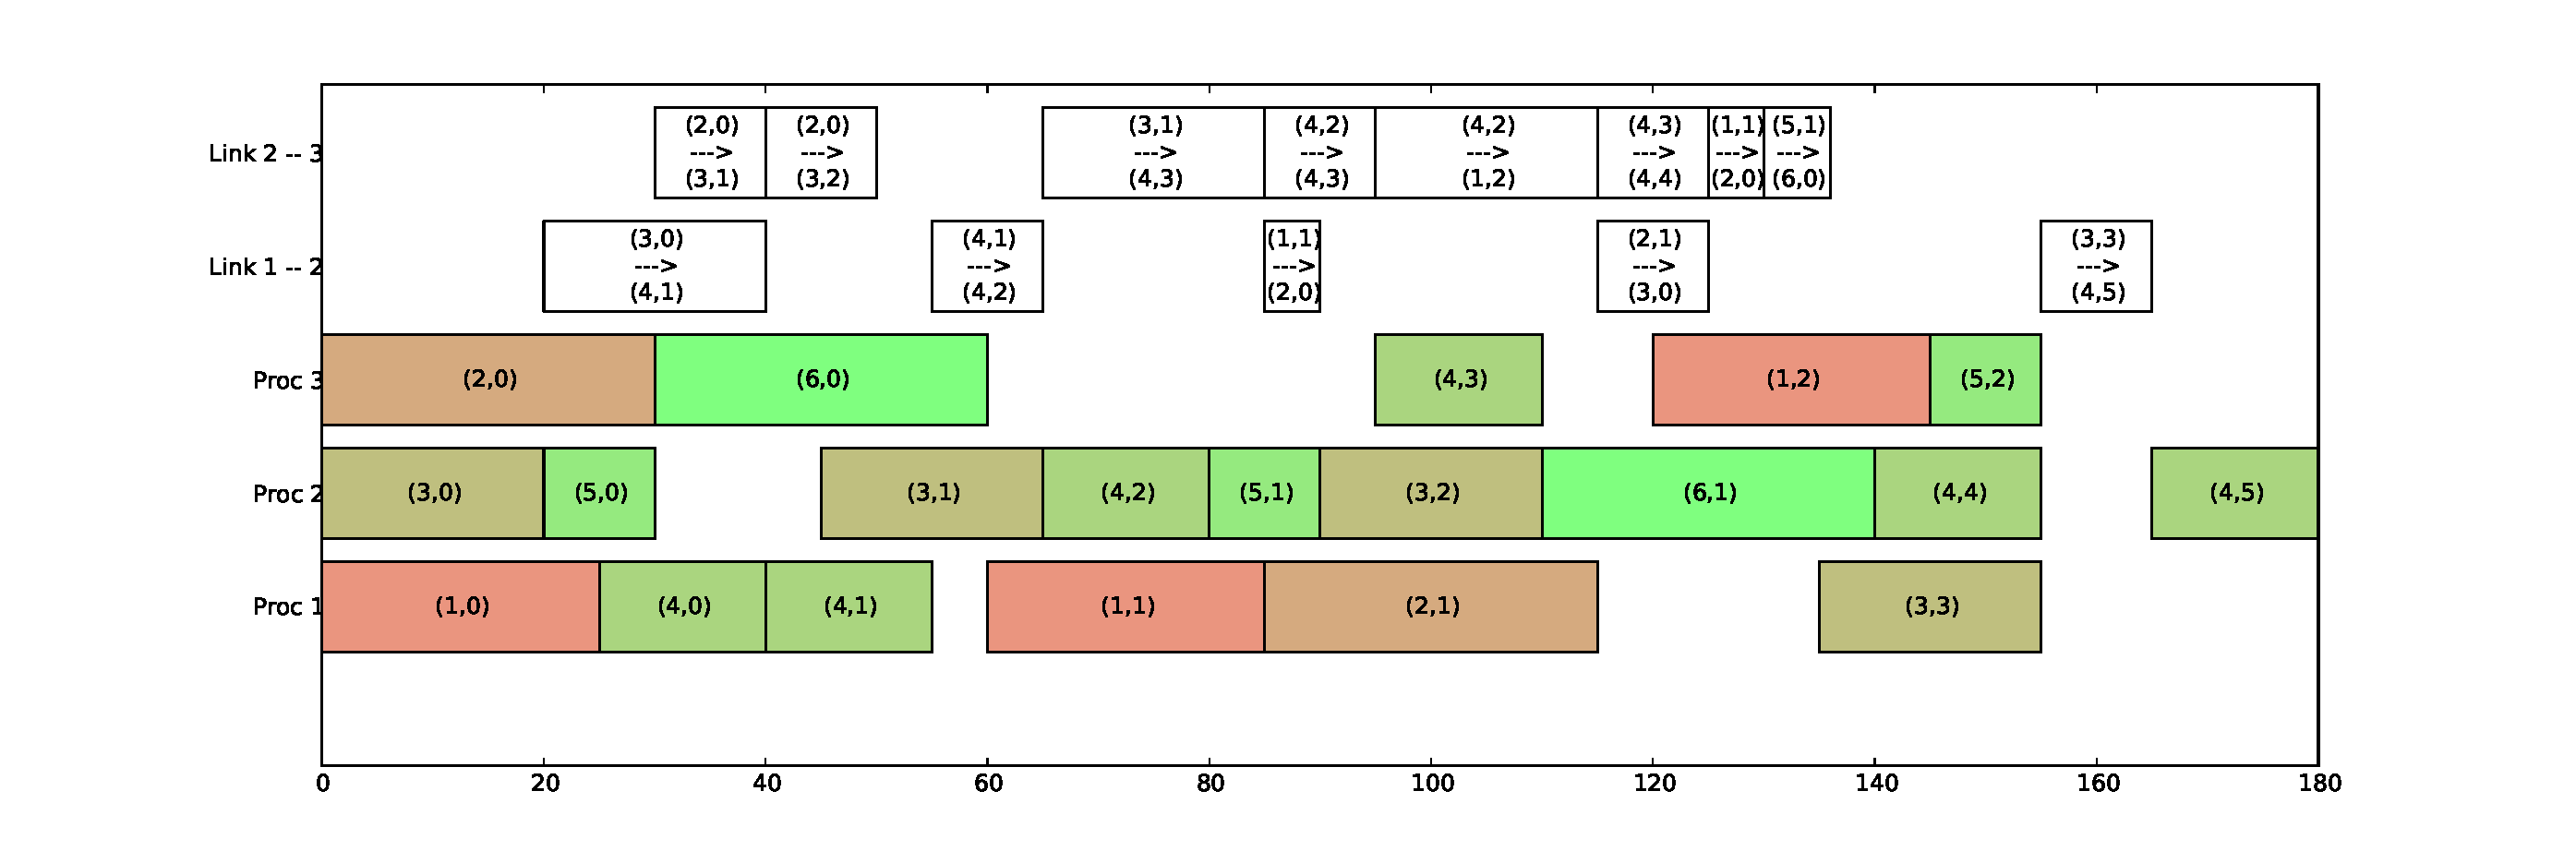
\includegraphics[width=40em]{figure/EXP-6task-sched2.pdf}\\
  \caption{添加自依赖后 6 个任务的调度表}\label{EXP-fig-6task-sched2}
\end{figure}

从图\ref{EXP-fig-6task-sched2}中可以看到任务4的执行区间 (4,0)、(4,1)、...、(4,5) 在时间上已不再有重叠,全部变为了串行执行,执行之间的通信开销也被考虑进了链路上的消息调度中。

\section{处理器排序对调度结果的影响}
下面我们来考察处理器排序对调度结果所造成的影响。在以上六个任务组成的任务集中,再添加三个任务,得到如表\ref{EXP-table-9task-time}所示的任务集,任务间的通信关系如图\ref{EXP-fig-9task-SDF}所示。其中 1---4 号任务和 7---9 号任务分别组成一个循环的通信关系,5号和6号任务组成单向的通信关系。
{\renewcommand{\arraystretch}{1.5}
\begin{table}
  \centering
  \caption{9个任务的时间约束}
  \label{EXP-table-9task-time}
  \begin{tabular}{|c|c|c|c|c|c|}
    \hline
    % after \\: \hline or \cline{col1-col2} \cline{col3-col4} ...
    任务 & 最坏执行时间$C_i$ & 周期$T_i$ & 偏移$O_i$ & 时间限$D_i$ & 自依赖\\
    \hline
    1 & 25 & 60 & 0 & 60 & 否\\
    2 & 30 & 0 & 0 & 0 & 否\\
    3 & 20 & 45 & 0 & 45 & 否\\
    4 & 15 & 0 & 0 & 0 & 否\\
    5 & 10 & 60 & 20 & 30 & 否\\
    6 & 30 & 0 & 0 & 0 & 否\\
    7 & 20 & 36 & 0 & 36 & 否\\
    8 & 30 & 0 & 0 & 0 & 否\\
    9 & 20 & 0 & 0 & 0 & 否\\
    \hline
  \end{tabular}
\end{table}
}
\begin{figure}[!hbt]
  \centering
  % Requires \usepackage{graphicx}
  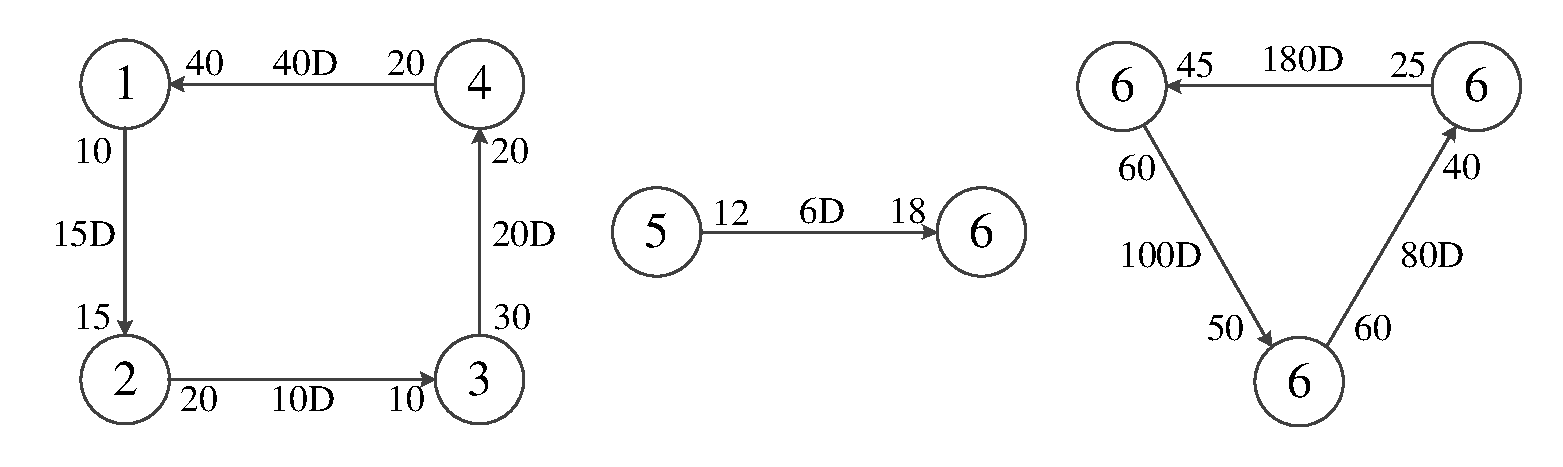
\includegraphics[height=24ex]{figure/EXP-9task-SDF.pdf}\\
  \caption{9个任务的 SDF 图}\label{EXP-fig-9task-SDF}
\end{figure}

在由7个处理器组成的目标平台上,处理器之间的拓扑连接如图\ref{EXP-fig-7p-link}所示。7 号处理器处于中枢位置,与其余 6 个处理器都相连,此外 1 和 2 号以及 4 号和 5 号处理器也分别相连。处理器之间的数据传输速率依然设为 1。
\begin{figure}[!hbt]
  \centering
  % Requires \usepackage{graphicx}
  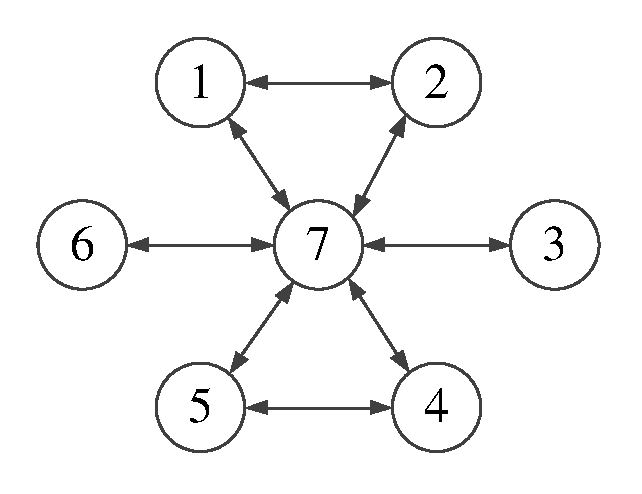
\includegraphics[height=20ex]{figure/EXP-7p-link.pdf}\\
  \caption{目标平台7个处理器间的拓扑连接}\label{EXP-fig-7p-link}
\end{figure}

将以上信息构建输入调度算法模拟程序,可以得到如图\ref{EXP-fig-9task}所示的调度表,说明此任务集可以调度。从以上处理器的托普连接可以看出,7号处理器的连接数是 6 为最多,其次是 1、2、4、5 号处理器,连接数均为 2,最后是 3 和 6 号处理器,连接数只有 1。按照处理器排序的情况下,程序的搜索顺序即为 7、1、2、4、5、3、6,当任务的开始时间相同时,且消息传递跳数相同的情况下,任务倾向于排布在靠前的处理器上,处理器之间连接通畅,易于消息调度。
\begin{figure}[!hbt]
  \centering
  % Requires \usepackage{graphicx}
  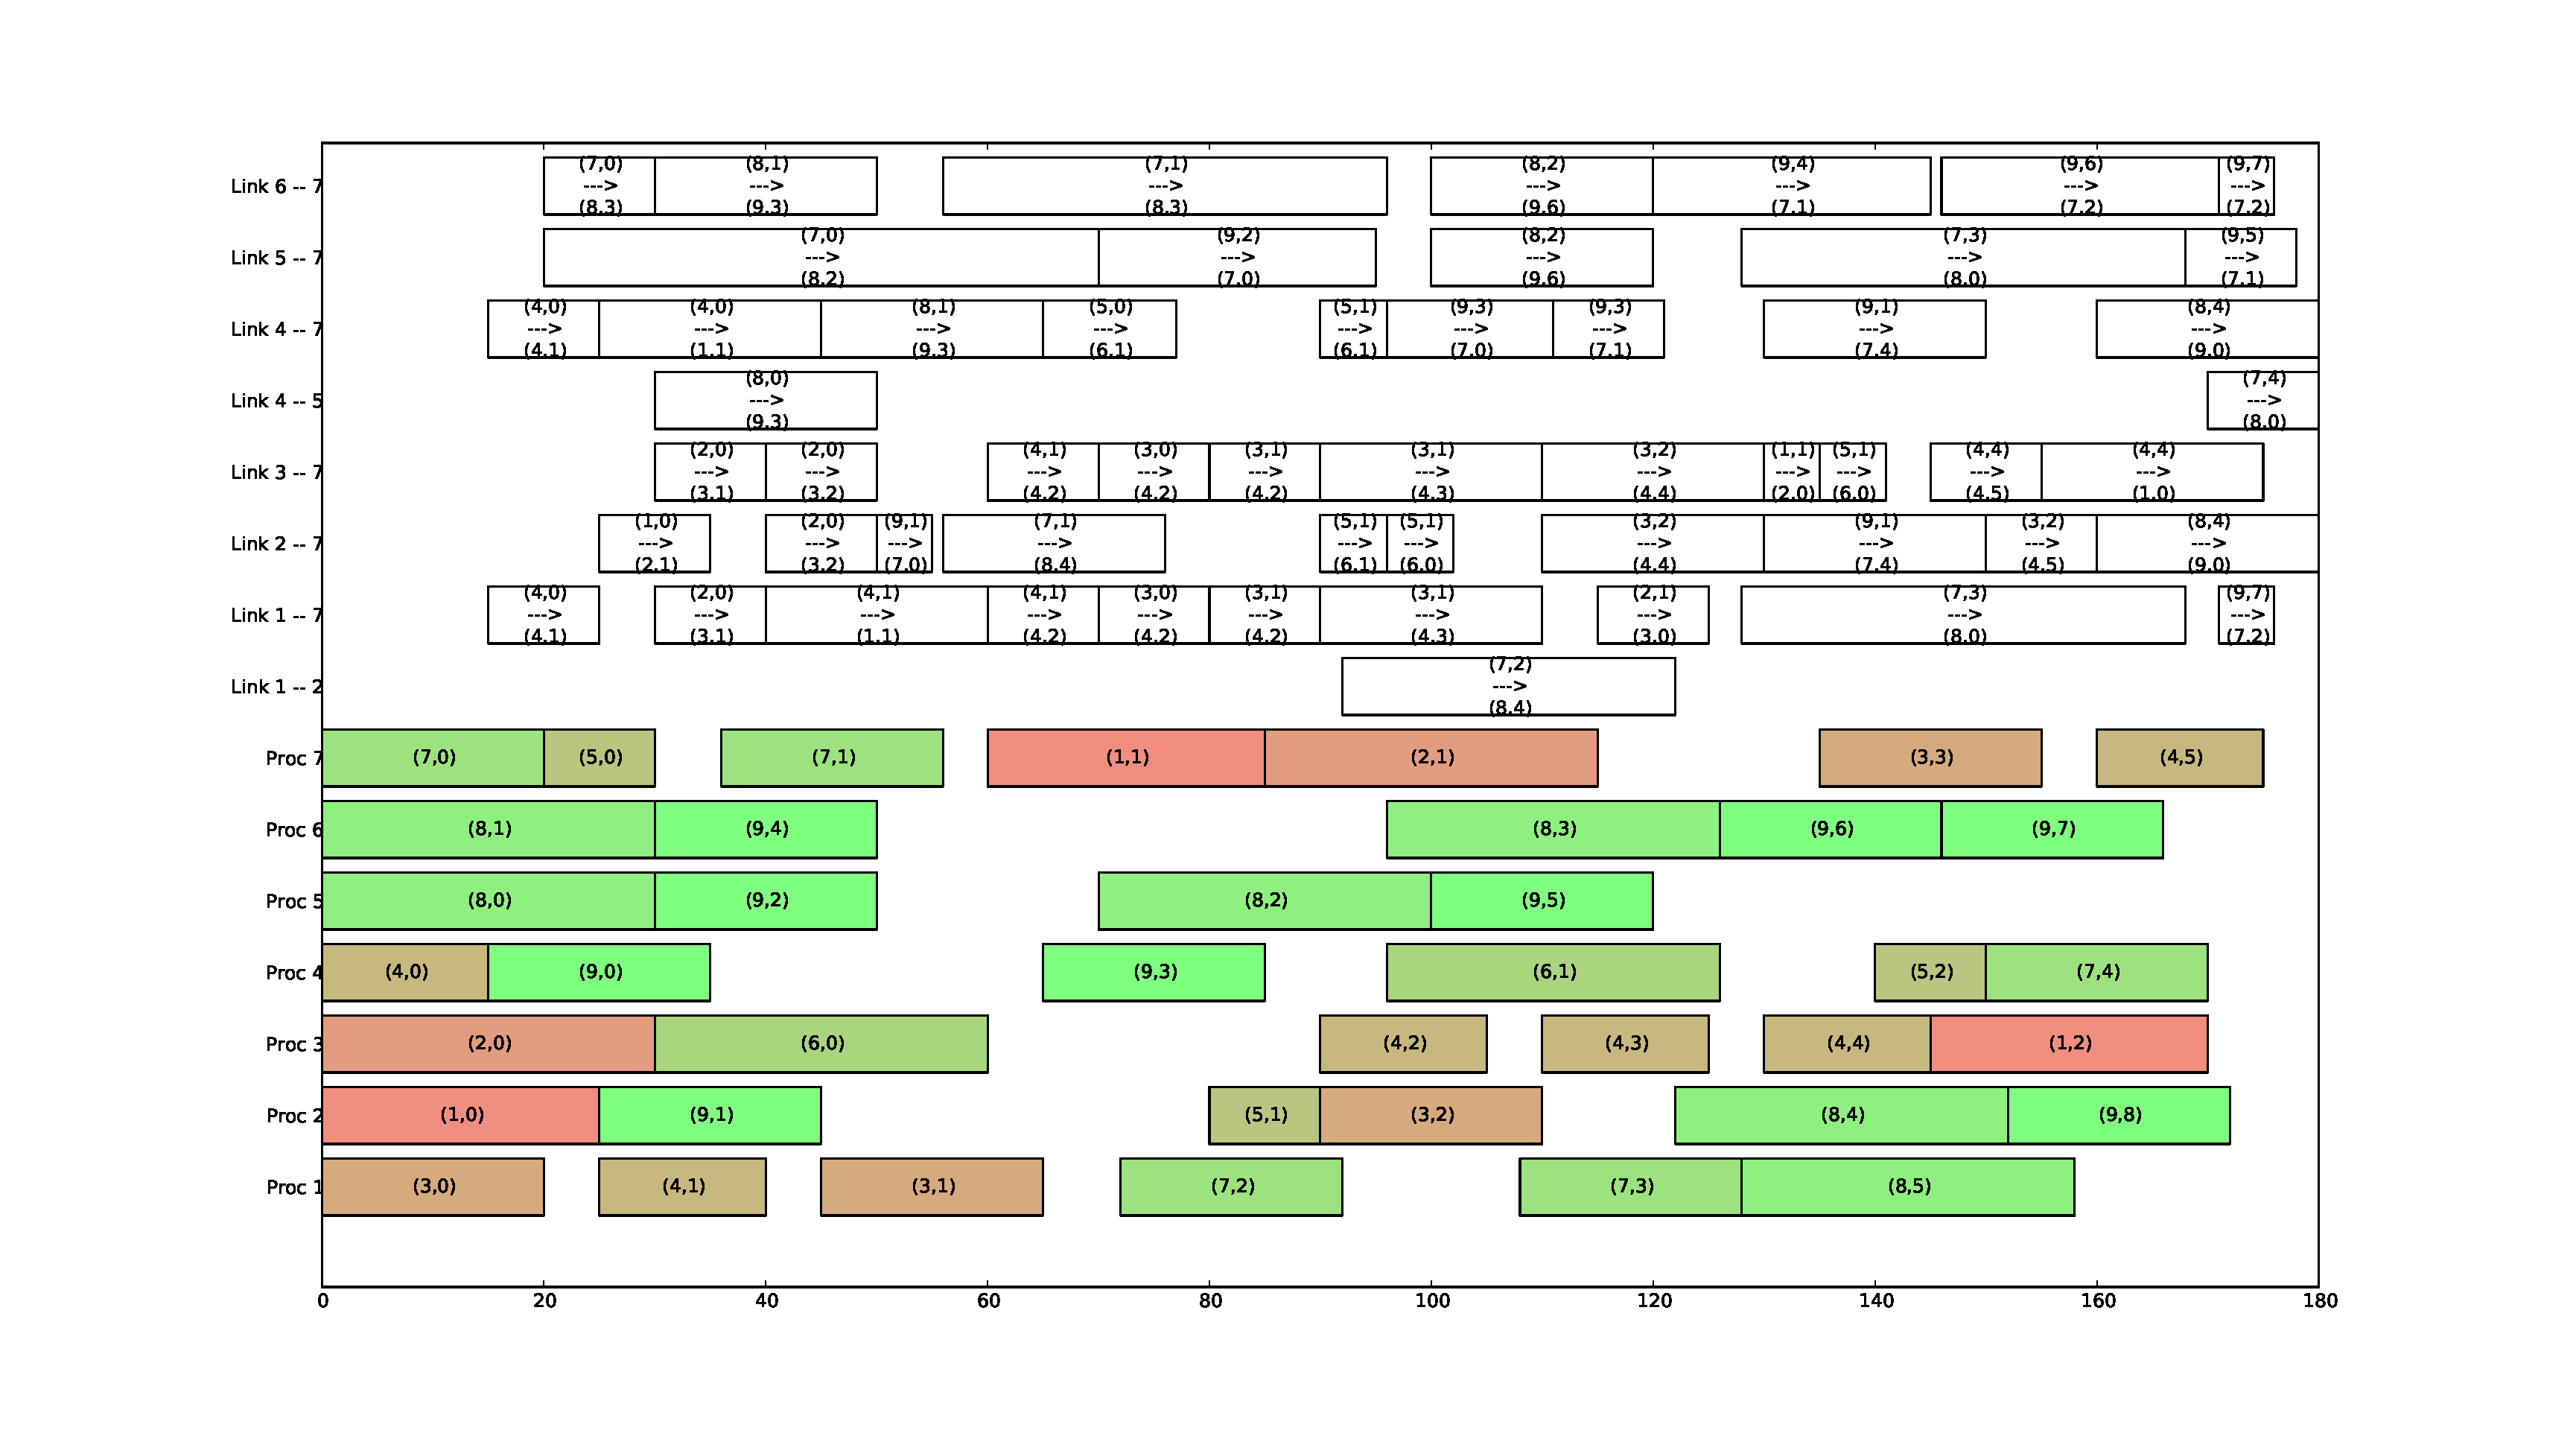
\includegraphics[width=40em]{figure/EXP-9task-sched.pdf}\\
  \caption{9个任务的调度表}\label{EXP-fig-9task}
\end{figure}

如果我们在程序中去除处理器排序部分,使得搜索仅仅按照处理器的序号依次进行。此时,当任务被排在 3 或 4 号结点均可时,未对处理器排序的情况下会将任务排在 3 号处理器上,那么此任务与其他处理器的通信都要经过 7 号处理器,通信较频繁的情况下会造成该链路上消息拥塞,难以调度开。如在上例中,去掉处理器排序后算法模拟程序即无法得到调度结果。

\section{本章小结}

本章首先用例子演示了模拟程序的计算流程,各步的具体结果,并结合最终产生的调度表分析验证了调度结果满足任务的时间及通信约束。本章第二个例子验证了任务的自依赖约束对调度结果产生的影响,最后一个例子验证了处理器排序优化在某些情况下有助于调度过程的搜索。
